\documentclass{iftex2024}
\usepackage{float}
\usepackage{ragged2e}
\renewcommand{\bibfont}{\justifying} %
\addbibresource{referencias.bib}
\titulo{APLICAÇÃO DE UMA META-HEURÍSTICA PARA OTIMIZAÇÃO DE PONTOS DE SAÍDA DE OPERAÇÕES EM NEGOCIAÇÕES ENVOLVENDO O MINICONTRATO FUTURO DO ÍNDICE BOVESPA}
\autor{Artur Francisco Pereira Carvalho}
\local{Bambuí -- MG}
\data{2024-12-11}

\campus{\textit{Campus} Bambuí}
\curso{Bacharelado}{Engenharia de Computação}
\titulacao{Bacharel}

\orientador{Prof. Dr. Ciniro Aparecido Leite Nametala}
\membrobanca{Marcos Roberto Ribeiro}{IFMG – Campus Bambuí}
\membrobanca{Matheus Clemente de Souza}{IFMG – Campus Bambuí}
\fichacatalografica{ficha.pdf}
\assinaturas{assinaturas.pdf}

\resumo{%
Este trabalho propõe a aplicação de uma meta-heurística para otimizar os pontos de saída de operações no mercado financeiro. 
A técnica utilizada é a Otimização por Enxame de Partículas (PSO). O estudo é focado no Minicontrato Futuro 
do Índice Bovespa (WINFUT). O objetivo é maximizar o retorno e minimizar o risco através da definição de pontos de \textit{stop-loss} e
\textit{take-profit} ideais. Utilizando uma estratégia baseada no cruzamento de médias móveis, o
algoritmo PSO é empregado para otimizar as operações de negociação. A pesquisa adota
uma abordagem quantitativa e experimental, combinando análise de dados históricos com
simulações para validar a eficácia da estratégia proposta. Os resultados são comparados
com uma estratégia de proporção fixa de 3:1, comum em plataformas de negociação,
destacando a eficácia do método desenvolvido.
}
\palavraschave{Otimização por Enxame de Partículas, PSO, Minicontrato Futuro do
Índice Bovespa, \textit{Stop-loss}, \textit{Take-profit}, Algoritmos de Otimização}

\abstract{%
This paper proposes the application of a metaheuristic to optimize the exit points of operations in the financial market. The technique used is Particle Swarm Optimization (PSO). The study focuses only on the Mini Futures Contract of the Bovespa Index (WINFUT). The objective is to maximize return and minimize risk by defining ideal stop-loss and take-profit points. Using a strategy based on the crossover of moving averages, the PSO algorithm is employed to optimize trading operations. The research adopts a quantitative and experimental approach, combining historical data analysis with simulations to validate the effectiveness of the proposed strategy. The results are compared with a fixed ratio strategy of 3:1, common in trading platforms, highlighting the effectiveness of the developed method.
}
\keywords{Particle Swarm Optimization, PSO, Mini Bovespa Index Futures, Stop-loss,
Take-profit, Optimization Algorithms.}

\listasiglas{%
 \begin{itemize}[]
  \item[B3] -- Brasil, Bolsa, Balcão
  \item[IFMG] -- Instituto Federal de Educação, Ciência e Tecnologia de Minas Gerais
  \item[WINFUT] -- Minicontrato Futuro do Índice Bovespa
  \item[TP] -- \textit{Take-Profit}
  \item[SL] -- \textit{Stop-Loss}
  \item[PSO] -- \textit{Particle Swarm Optimization}
  \item[SMA] -- \textit{Simple Moving Average}
  \item[LSTM] -- \textit{Long Short-Term Memory}
  \item[GGA] -- \textit{Genetic Grouping Algorithm}
  \item[ATR] -- \textit{Average True Range}
  \item[PE] -- Pregão Eletrônico
  \item[PVV] -- Pregão Viva Voz
 \end{itemize}
}

\begin{document}

\maketitle

\chapter{INTRODUÇÃO}

As negociações nos mercados financeiros, que antes eram realizadas em salas ocupadas por 
operadores humanos nos chamados `Pregão Viva Voz' (PVV), já não existem atualmente. 
Nas últimas décadas, houve uma informatização intensiva dos
mercados financeiros, substituindo operadores humanos por algoritmos automatizados.
Embora esses algoritmos sejam criados por pessoas, as decisões sobre quando enviar ordens
de compra ou venda são tomadas pelos próprios algoritmos e executadas automaticamente
por meio de uma infraestrutura tecnológica que conecta empresas comerciais individuais às
várias bolsas onde negociam. Isso transformou significativamente a natureza dos mercados
financeiros e o funcionamento das organizações envolvidas. Além de reformular a relação
entre humanos e tecnologia na indústria financeira, essa mudança atualizou os mercados
através de arranjos sociotécnicos que permitem a interação entre agentes humanos e
não-humanos \cite{bointroducao}.

O mercado financeiro é influenciado por diversos fatores macroeconômicos e
microeconômicos, incluindo a conjuntura econômica geral, eventos políticos, expectativas
dos investidores institucionais, decisões de especuladores individuais e as estratégias
operacionais das empresas comerciais. No entanto, os impactos específicos desses fatores
sobre o sistema financeiro, que é dinâmico por natureza, ainda não são completamente
compreendidos. Isso torna a previsão de dados financeiros desafiadora, devido à incerteza
externa e à complexidade intrínseca envolvida \cite{TANG2022363}.

O gerenciamento de risco no mercado financeiro é uma tarefa 
complexa, dada a sua relação direta com a estabilidade financeira
e a viabilidade econômica das empresas. A realização de atividades empresariais está
intrinsecamente associada a riscos, sendo que as entidades empresariais frequentemente
obtêm maiores lucros ao se envolverem em atividades com níveis elevados de risco \cite{Pakhucha_Sievidova_Siadrysta_Mohilevsky_Oliynik_Bogdanovych_2021}. No
entanto, isso também aumenta a ameaça de perda da estabilidade financeira. O risco
financeiro, classificado como um risco especulativo, envolve a possibilidade de resultados
tanto negativos quanto positivos, e é influenciado por um conjunto complexo de relações
de causa e efeito. 

A situação econômica instável e a rápida introdução de novas
tecnologias e instrumentos financeiros amplificam a importância dos riscos financeiros
nas atividades econômicas e financeiras. Portanto, a identificação e a avaliação precisa
dos riscos financeiros são essenciais para mitigar perdas potenciais e assegurar recursos
financeiros adicionais, garantindo que o investidor alcance seus objetivos e supere os
desafios ao longo de seu ciclo de vida \cite{Pakhucha_Sievidova_Siadrysta_Mohilevsky_Oliynik_Bogdanovych_2021}. Dada a relevância do
gerênciamento de risco, este trabalho tem como intuito a mitigação riscos em operações
no mercado financeiro.

\section{Justificativa e proposta}

O mercado financeiro, com sua natureza altamente volátil, representa um desafio
significativo para investidores que buscam maximizar retornos enquanto minimizam riscos.
Em particular, o Minicontrato Futuro do Índice Bovespa (WINFUT) tem se destacado
como um instrumento para investidores devido à sua capacidade de proporcionar
alavancagem e oportunidades de lucro em diferentes condições de mercado. Em alguns
estudos, como em \textcite{bovespa1} e \textcite{bovespa2}, são aplicadas técnicas de 
previsão de séries temporais no WINFUT para auxiliar na tomada de decisão e reduzir a exposição ao risco,
ilustrando a relevância do WINFUT no contexto de estratégias de investimento. No
entanto, a volatilidade inerente e as rápidas oscilações de preço dificultam a gestão eficiente
desses investimentos.

Duas estratégias envolvendo pontos de saída são comumente utilizadas: \textit{stop-loss} (SL) e \textit{take-profit} (TP), 
ambas relacionadas à saída do mercado por parte do investidor. O SL ocorre quando o preço do ativo atinge um nível 
desfavorável, enquanto o TP é acionado quando o preço atinge um nível suficientemente favorável.
O uso dessas estratégias é uma prática comum para gerenciar riscos e assegurar lucros \cite{WOS:000231777300003}. 
No entanto, estudos como o de \textcite{Santos_Silva_Villagrán_Ribeiro_Sanfins_2021}, ressaltam a dificuldade de alcançar retornos satisfatórios com
riscos mínimos, evidenciando a necessidade de métodos mais robustos e sistemáticos para
otimizar decisões de negociação.

Nesse contexto, a aplicação de algoritmos de otimização meta-heurísticos, como
o \textit{Particle Swarm Optimization} (PSO), conhecido em português como Otimização por Enxame de Partículas \cite{488968}, emerge como uma solução promissora.
Esses algoritmos, inspirados em fenômenos naturais e biológicos, são capazes de explorar
eficientemente o espaço de busca, evitando ótimos locais e buscando soluções globais. O
PSO, em particular, tem demonstrado eficácia em diversos domínios de otimização devido
à sua capacidade de adaptar dinamicamente ao problema em questão \cite{PSO25ANOS}.

A proposta deste trabalho é desenvolver um modelo de otimização baseado no
PSO para determinar pontos ideais de saída em operações de negociação com o WINFUT. O
algoritmo foi projetado para lidar com números de ponto flutuante.
O processo de otimização envolverá a análise do histórico de preços do WINFUT,
combinado com a simulação de operações com o ativo por meio da geração de sinais de compra,
que foram definidos utilizando uma estratégia baseada no cruzamento
de médias móveis. A partir destes sinais foi realizado a otimização dos
pontos de saída pelo algoritmo PSO, para maximizar os retornos e minimizar as perdas. Com os pontos
de saída definidos, foi feito uma comparação entre o pontencial de retorno dessa abordagem
em relação a uma estratégia já consolidada.

\section{Objetivos}

Este estudo propõe atender ao objetivo geral e aos objetivos específicos descritos
a seguir.

\subsection{Objetivo geral}

Obter, por meio da implementação do algoritmo de otimização meta-heurística PSO, os pontos ótimos de saída, 
que neste estudo serão definidos pelo SL e TP, nas negociações do ativo WINFUT, 
de forma a alcançar a relação ideal entre risco e retorno para operar nesse ativo.

\subsection{Objetivos específicos}

\begin{itemize}
  \item Obtenção do histórico de preços do minicontrato futuro do índice Bovespa.
  \item Relizar o cálculo das médias móveis nos preços obtidos, para definição de pontos de compra e venda.
  \item Implementar o algoritmo PSO para definir os valores ótimos de TP e SL,
  em que nele seja maximizado o lucro nas negociações a partir dos pontos de compra
  definidos.
  \item Avaliar os resultados obtidos pelo algoritmo de otimização e comparar com uma estratégia já utilizada no mercado.
\end{itemize}

\subsection{Características da pesquisa}

No que tange a metodologia científica esta pesquisa está caracterizada da
seguinte forma:

\begin{enumerate}
  \item Quanto a finalidade: É uma pesquisa aplicada, visto que propõe o estudo e
  desenvolvimento de um algoritmo de otimização para resolver problemas específicos na área
  de negociação financeira, envolvendo a definição de pontos de saída para o minicontrato
  futuro do índice Bovespa;
  \item Quanto ao objetivo: É uma pesquisa exploratória, pois investiga e combina
  diferentes técnicas (PSO e médias móveis) para otimização de pontos de saída;
  \item Quanto a abordagem: É uma pesquisa quantitativa, visto que todas as
  decisões de implementação são guiadas por métricas numéricas, uma vez que envolve o
  uso de algoritmos e técnicas de otimização para definir pontos de TP e SL
  com base em dados históricos de mercado.
  \item Quanto ao método: É uma pesquisa experimental, pois testa a aplicação
  do PSO combinado com médias móveis em dados históricos do mercado financeiro para
  avaliar a eficácia da estratégia proposta. Este método envolve a realização de simulações e
  testes empíricos para validar os resultados.
 \end{enumerate}

\section{Estrutura do documento}

Este trabalho está organizado em seis capítulos que abordam o desenvolvimento e a aplicação de uma meta-heurística 
para otimização de pontos de saída em negociações com o Minicontrato Futuro do Índice Bovespa:

\begin{itemize}
  \item Capítulo 1 - Introdução: Apresenta a motivação, a justificativa e os objetivos 
  do estudo, fornecendo uma visão geral sobre a relevância da otimização de pontos de saída no 
  contexto do mercado financeiro.
  \item Capítulo 2 - Fundamentação Teórica: Descreve os principais conceitos relacionados ao 
  mercado financeiro, negociação algorítmica, e técnicas de análise técnica, além de uma revisão dos 
  algoritmos de otimização, com ênfase no PSO. 
  \item Capítulo 3 - Revisão Bibliográfica: Analisa o estado da arte nas técnicas para definir SL e 
  TP em negociações, destacando abordagens semelhantes ao trabalho proposto e apresentando o diferencial da metodologia adotada.
  \item Capítulo 4 - Metodologia: Detalha os procedimentos adotados para coleta e tratamento dos dados, a definição 
  das simulações de compra com médias móveis e a implementação do algoritmo PSO para otimização dos pontos de saída.
  \item Capítulo 5 - Resultados: Apresenta e discute os resultados obtidos com a aplicação do PSO e as comparações entre 
  diferentes abordagens, evidenciando o desempenho da metodologia proposta.
  \item Capítulo 6 - Conclusão: Resume as contribuições e as principais descobertas do estudo, sugerindo direções para 
  futuras pesquisas e aplicações práticas da abordagem desenvolvida.
\end{itemize}

\chapter{FUNDAMENTAÇÃO TEÓRICA}

Neste capítulo é apresentada uma contextualização acerca do ambiente no
qual se aplica o objeto de estudo da pesquisa. Iniciando-se pela grande área de mercado
financeiro, serão apresentados conceitos fundamentais que visam munir o leitor sobre o
funcionamento das negociações de ativos e o papel econômico que estas desempenham.
Na sequência, com foco apenas no minicontrato futuro do índice Bovespa, é feita uma
abordagem sobre os contratos futuros e sobre o Índice Bovespa. Logo em seguida estão
as seções diretamente ligadas as formas de operação no mercado, onde é apresentado
a relação entre risco e retorno, a negociação algorítmica, e a estratégia de negociação
baseada no cruzamento de médias móveis. A seção é complementada por uma descrição
dos algoritmos de otimização, conceituando e abordando os agrupamentos dos métodos
de otimização. Ao final, é abordado o PSO.

\section{Mercado financeiro}

O sistema financeiro é composto por diversas instituições e instrumentos financeiros que permitem a movimentação de recursos dos fornecedores finais para os consumidores
finais, além de garantir que títulos e valores mobiliários possam ser convertidos em dinheiro
no mercado \cite{cavalcante2009mercado}.

Até o início da década de 1990, a bolsa de valores brasileira, conhecida na
época como BOVESPA, utilizava principalmente o método de Pregão Viva Voz (PVV)
para realizar transações entre investidores. Em 1999, foi introduzido o sistema de 
\textit{Home Broker}, que são \textit{softwares} que permitem que os investidores enviem ordens de compra e venda ao
mercado por meio da corretora escolhida. A adoção do \textit{Home Broker} possibilitou a
intermediação eletrônica de operações pelas corretoras, levando à substituição do PVV
pelo pregão eletrônico (PE) que era utilizado em bolsas de valores ao redor do mundo
\cite{nametala2017construccao}.

Em março de 2017, a BM\&FBOVESPA, que surgiu em 2008 da união entre
BM\&F e Bovespa Holding, também se uniu a Cetip com um propósito em comum de
trabalhar para conectar, desenvolver e viabilizar o mercado financeiro e de capitais,
formando assim a B3 S.A. - Brasil, Bolsa, Balcão \cite{B3}.

\section{Minicontrato Futuro do Índice Bovespa}

Os contratos futuros juntamente com as opções compõem o tipo de contrato chamado derivativo, estes são
negociados ativamente em muitas bolsas de todo o mundo, a definição de derivativo envolve
ser um instrumento financeiro que deriva de valores de outras variáveis subjacentes mais
básicas, onde muitas vezes estas variáveis são preços de ativos negociados. Entretanto, os
derivativos podem depender tanto de fatores como preço de uma \textit{commoditie} quanto de
fatores climáticos de uma região \cite{hull2016opccoes}.

O Índice Bovespa (Ibovespa) é uma carteira teórica de ativos que mede o
desempenho das ações mais representativas do mercado brasileiro. Atualmente, ele é
considerado um termômetro do cenário político e econômico do país. O Ibovespa é revisado
a cada quatro meses, com base na liquidez das ações nos últimos doze meses, dando maior
peso às empresas mais líquidas. Utilizado como referência para cálculos de risco e beta,
inclui apenas ativos listados na B3. Para investidores, o Ibovespa
serve como parâmetro de desempenho, sendo ideal que a carteira alcance um desempenho
igual ou superior ao índice \cite{nunes2020relaccao}.

\section{Relação risco e retorno}

Risco e retorno são conceitos essenciais no mundo dos investimentos. O risco
envolve à avaliação dos perigos individuais, incorporando a compreensão das interações
entre diferentes ativos, expressas por meio das covariâncias e variâncias. Enquanto o retorno
de um investimento é geralmente determinado de maneira mais direta. Ele representa o
montante total de lucros ou prejuízos obtidos ao longo de um determinado intervalo de
tempo \cite{NETORISCO}.

De acordo com \textcite{WOS:000231777300003}, entre as abordagens mais utilizadas
no mundo dos investimentos, para lidar eficazmente com as incertezas envolvidas nas
negociações de ações, futuros e outros ativos, estão as estratégias baseadas em preços para
entrar ou sair do mercado. A seguir, estão duas das principais abordagens que estão entre
as mais utilizadas nessas estratégias.

\begin{itemize}
  \item \textit{Stop-loss} (SL): Ordens de \textit{stop-loss} são utilizadas para limitar as perdas. Quando o
  preço de um ativo atinge um nível desfavorável, o investido sai do mercado aceitando
  o prejuízo atual, de forma a evitar um resultado ainda pior.
  \item \textit{Take-profit} (TP):  Metas de lucro são usadas para garantir ganhos. Quando o preço
  se torna suficientemente favorável, o investido sai do mercado e reavalia a situação,
  possivelmente acreditando que o mercado está inflacionado e prestes a passar por
  uma correção.
\end{itemize}

\section{Negociação algorítmica}

Para dar suporte as negociações no mercado, surgiu a negociação algorítmica que é definida por 
\textcite{hendershott2012algorithmic}, como a automação do processo
de tomada de decisões de negociação, que inclui a submissão de ordens ao mercado e o
gerenciamento das respostas a essas ordens, tudo isso realizado por meio de algoritmos
computacionais. Outra definição é dada por \textcite{portnoy2011high}, que diz que a negociação
algorítmica envolve examinar estatisticamente o histórico de um ativo específico, considerando 
também as condições atuais do mercado. Seu objetivo é prever a direção dos
movimentos nos preços e identificar oportunidades de lucro através de operações baseadas
nessas previsões.

Uma decisão de investimento de mercado pode ser complexa devido a incerteza da tarefa e à sua alta dinâmica, 
ou seja, uma estratégia que estava correta no momento t não é correta no momento t + 1. 
Assim, para tais tarefas, dois estágios são necessários para o desenvolvimento dos algoritmos: imitar o processo
de decisão humana em um alto nível, e imitar o funcionamento do cérebro humano para
reproduzir essa boa decisão \cite{WILINSKI2017100}.

\section{Médias móveis}

As médias móveis formam uma das construções estatísticas que são
utilizadas na negociação nos mercados financeiros de todos os tipos, ações mais
do que outros, em uma variedade de diferentes interpretações de estratégias (ou regras) de
negociação. Sendo um elemento básico de negociação na análise técnica, suas propriedades e eficácia foram consideradas 
em muitos estudos acadêmicos anteriores \cite{PAPAILIAS2015458}.

A equação (\ref{eq:mediasMoveis}) representa como a \textit{Simple Moving Average} (SMA) conhecia em português como média móvel simples do preço, é calculada. 
Esta média é móvel porque, no final de cada período de negociação, 
é adicionado o período mais recente e descartado o período mais antigo da média anterior.

\begin{equation}
  \label{eq:mediasMoveis} 
  \text{SMA}_n = \frac{1}{n} \sum_{i=0}^{n-1} P_{t-i}   
\end{equation}

\noindent{em que:}
\begin{itemize}
  \item $\text{SMA}_n$ é a Média Móvel Simples no período $n$,
  \item $n$ é o número de períodos,
  \item $P_{t-i}$ é o preço de fechamento no segundo $t-i$.
\end{itemize}

De acordo com \textcite{el2009decision}, um dos indicadores de estratégia de investimento relacionado a análise 
técnica que gera um maior retorno baseado no movimento do histórico de preços é o cruzamento de médias móveis. 
O principal conceito por trás da média móvel é calcular a média de um número \textit{n} de pontos/preços de dados anteriores. 
Esta média calculada representa a área de preço mais próxima de um número proporcionalmente grande de negociações naquele 
período especificado. O cruzamento de médias móveis é dado quando o valor de uma média de curto prazo encontra 
com uma de longo prazo.

A figura \ref{figura:cruzamento de médias móveis} mostra o gráfico de preços de fechamento para o ativo WINQ24
(Mini índice Bovespa no ano de 2024) em um período de 300 segundos, com o cálculo de duas SMA’s. 
Uma rápida (em amarelo) de 9 segundos e outras lenta (verde) de 21 segundos.

\begin{figure}[!htb] \centering
  \caption{Cruzamento de médias móveis} \label{figura:cruzamento de médias móveis}
  \begin{varwidth}{\linewidth}
    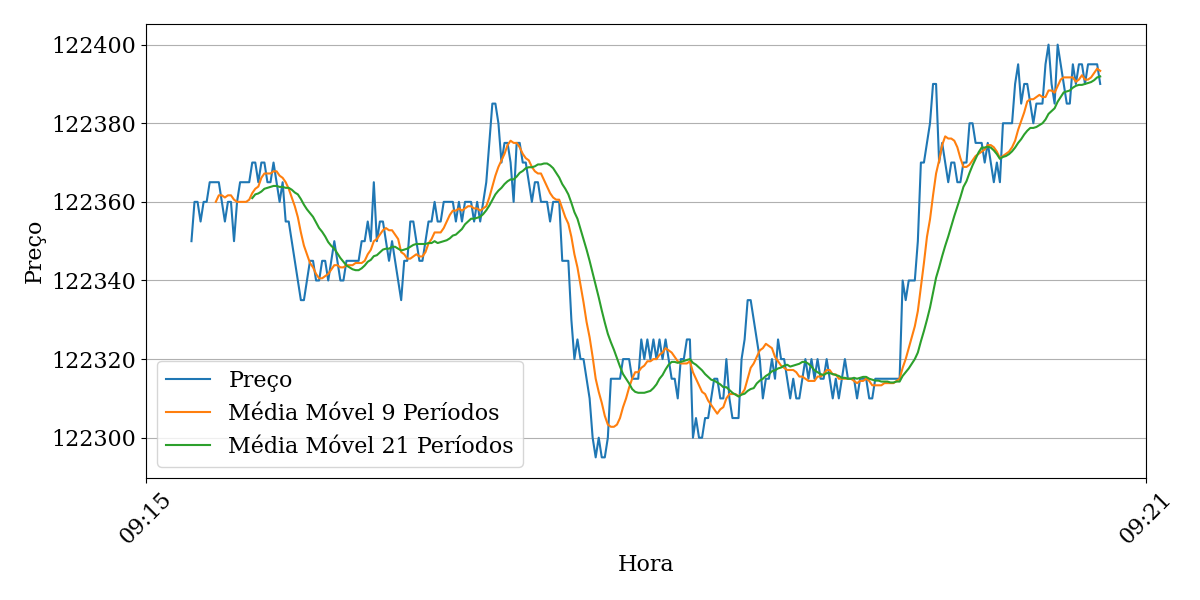
\includegraphics[width=14cm]{figuras/tccCruzamento média móvel.png}
    \legend{Elaborado pelo Autor, 2024.}
  \end{varwidth}
\end{figure}

\begin{figure}[!htb] \centering
  \caption{Estratégia preço x média móvel} \label{figura:estrategia1}
  \begin{varwidth}{\linewidth}
    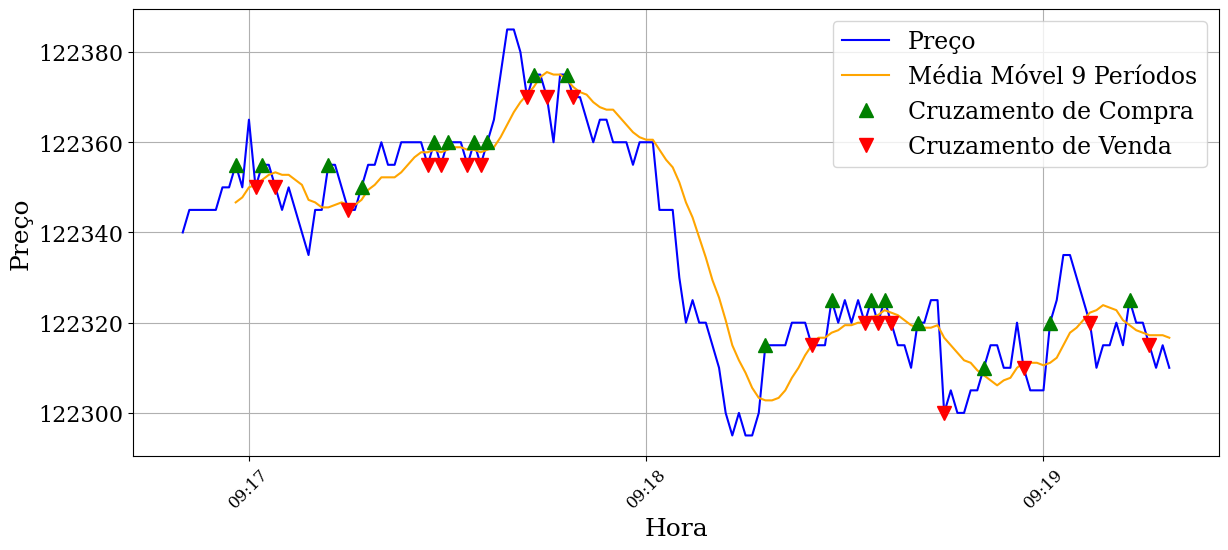
\includegraphics[width=14cm]{figuras/estrategia1.png}
    \legend{Elaborado pelo Autor, 2024.}
  \end{varwidth}
\end{figure}

\begin{figure}[!htb] \centering
  \caption{Estratégia média móvel lenta x média móvel rápida} \label{figura:estrategia_2}
  \begin{varwidth}{\linewidth}
    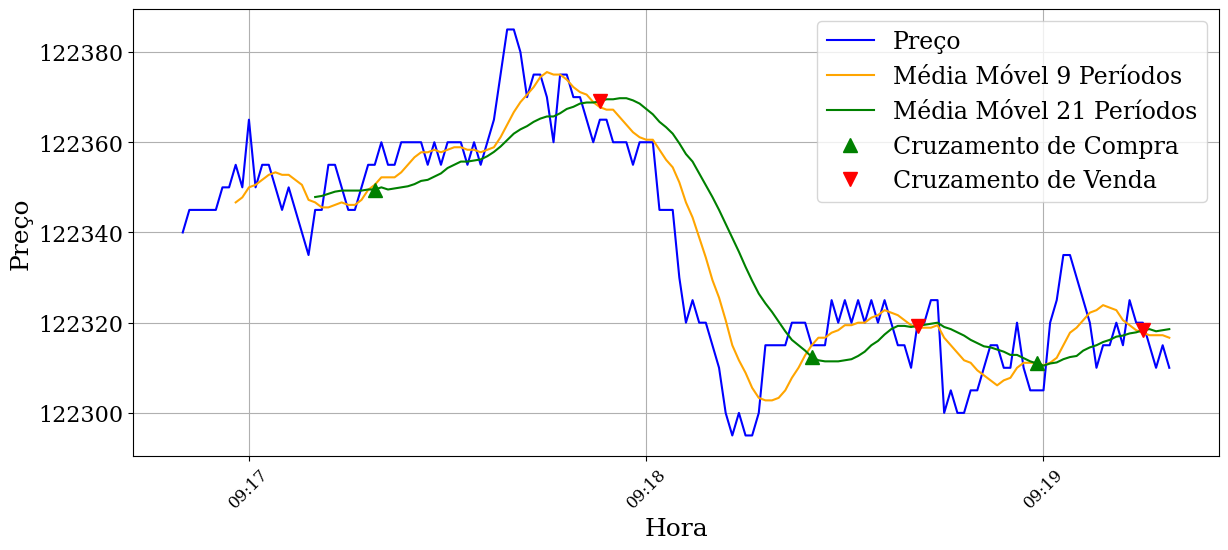
\includegraphics[width=14cm]{figuras/estrategia2.png}
    \legend{Elaborado pelo Autor, 2024.}
  \end{varwidth}
\end{figure}

Duas das estratégias para negociação que fazem uso de médias móveis baseiam-se no cruzamento de preços e no cruzamento 
de médias móveis. A primeira estratégia, representada na figura \ref{figura:estrategia1}, emite um sinal para realizar 
a compra de um ativo quando o preço do ativo ultrapassa a SMA, enquanto a segunda estratégia, 
representada na figura \ref{figura:estrategia_2}, emite o sinal de compra  quando uma SMA mais rápida 
cruza acima de uma SMA mais lenta. Os sinais para realização da venda do ativo comprado são definidos 
na direção oposta, ou seja, quando a SMA  mais lenta cruza acima de uma média 
móvel mais rápida \cite{PAPAILIAS2015458}.

\section{Algoritmos de otimização}

A otimização pode ser definida como um conjunto de técnicas e algoritmos utilizados para encontrar a melhor solução possível
dentro de um conjunto de alternativas viáveis, de forma iterativa. Esses métodos são amplamente empregados em problemas 
complexos, como aqueles de natureza combinatória, onde o objetivo é maximizar ou minimizar uma função de acordo com os 
critérios do problema \cite{castellifernando}.

Os primeiros métodos utilizados para resolver problemas de otimização eram
métodos matemáticos ou numéricos nos quais a solução final é determinada alcançando
um ponto onde a derivada da função é zero. Contudo, resolver problemas não lineares e
não convexos, que envolvem muitas variáveis e restrições, utilizando esses métodos se torna
praticamente impossível, especialmente à medida que o número de dimensões aumenta,
resultando em um espaço de busca que cresce exponencialmente. Além disso, os métodos
numéricos podem ficar presos em pontos de ótimos locais nos quais a derivada também é
zero. Isso implica que não há garantia de encontrar a solução ótima global ao empregar
tais métodos numéricos \cite{ZERVOUDAKIS2020106559}.

Segundo \textcite{MIRJALILI201651} os algoritmos de otimização por meta-heurística estão se popularizando 
em aplicações de engenharia pela capacidade de evitar ótimos locais e ampla aplicabilidade. Os algoritmos de 
meta-heurística inspirados na natureza resolvem problemas de otimização imitando fenômenos biológicos ou físicos. 
Eles podem ser agrupados em três categorias principais: 

\begin{itemize}
  \item Métodos baseados na evolução: Inspirados na evolução natural, começam com uma população aleatória que evolui ao longo das gerações, combinando os melhores indivíduos para otimização. Exemplos incluem Algoritmos Genéticos (GA) e Estratégia de Evolução (ES).
  \item Métodos baseados na física: Imitam regras físicas do universo. Exemplos incluem Recozimento Simulado (SA) e Algoritmo de Busca Gravitacional (GSA).
  \item Métodos baseados em enxames: Imitam o comportamento social de animais. Exemplos incluem Otimização por Enxame de Partículas (PSO) e Otimização por Colônia de Formigas (ACO).
\end{itemize}

\section{Otimização por Enxame de Partículas (PSO)}

Diversas aplicações de engenharia fazem uso de algoritmos de otimização para abordar problemas de forma eficiente 
e eficaz, resolvendo desafios específicos. Entre os problemas de otimização do mundo real, grande parte é solucionada 
por meio de algoritmos meta-heurísticos. Um desses algoritmos é o PSO, introduzido por \textcite{488968}. A ideia e a formulação do algoritmo PSO foram inspiradas 
pela observação do comportamento social de bandos de pássaros e cardumes de peixes, em que os integrantes do grupo seguem 
um líder que está mais próximo da comida. Esse comportamento social pode ser traduzido em operações algorítmicas, como 
no PSO, para resolver problemas de otimização, onde o bando de pássaros é representado como um enxame de partículas, 
e cada partícula corresponde a uma solução candidata. Durante a fase de exploração, as partículas percorrem o espaço 
de busca extensivamente, enquanto a fase de exploração foca em regiões promissoras \cite{WOS:000986168700001}.

O PSO é uma técnica de otimização que modela o conjunto de possíveis soluções de problemas como um conjunto de particulas
se movimentando em um espaço virtual. O método original do PSO consiste em 
um espaço vitual onde se instancia várias partículas formando um enxame e cada uma começa com uma
posição ($x_{i,j}$) e uma velocidade ($v_{i,j}$) aleatórias no espaço de busca \textit{n}-dimensional, onde \textit{i}
representa o índice da partícula e \textit{j} representa a dimensão no espaço de busca. As partículas
otimizam as soluções candidatas ao se movimentar através do espaço virtual, atraindo-se
para posições que resultaram nos melhores desempenhos \cite{WOS:000233683900013}.

As partículas são organizadas em vizinhanças, que facilitam a comunicação
entre as partículas enquanto buscam os pontos ótimos. Existem diversas topologias de enxame, ou sociometrias, como
estrela, anel, pirâmide e Von Neumann, e estas influenciam o desempenho do PSO. A
equação de atualização da velocidade é composta por três componentes: o termo de
\textit{momentum}, o termo cognitivo e o termo social. O termo de \textit{momentum} direciona o
movimento da partícula para continuar na direção do movimento anterior, facilitando
trajetórias mais suaves. O termo cognitivo orienta o movimento da partícula em direção a
áreas do espaço de busca que a partícula já encontrou como promissoras para um ótimo.
Por fim, o componente social direciona o movimento da partícula para áreas do espaço de
busca identificadas por qualquer partícula na vizinhança relevante como promissoras para
um ótimo. A melhor posição social de cada vizinhança é definida como a melhor posição
pessoal da partícula que encontrou o melhor resultado dentro daquela vizinhança \cite{math11132980}.

Muitos pesquisadores como \textcite{erwinPSO} e \textcite{CorreaPSO}, realizaram modificações no algoritmo original, resultando
em um grande número de variantes do PSO com desempenho aprimorado. As principais
estratégias de modificação incluem a alteração dos parâmetros de controle do PSO,
hibridização do PSO com outros algoritmos meta-heurísticos, e técnicas de cooperação e
multi-enxame. Algumas dessas variantes incluem o PSO binário, que adapta o
PSO para espaços de busca discretos, e topologias de vizinhança no PSO, que influenciam
como as partículas interagem e compartilham informações \cite{WOS:000986168700001}.

\chapter{REVISÃO BIBLIOGRÁFICA}

Este capítulo faz uma revisão bibliográfica que tem por objetivo apresentar o
estado da arte. Inicialmente é feito uma
introdução às principais técnicas utilizadas para definir pontos de saída de operações em
negociações no mercado financeiro. Concluindo a revisão, será abordado sobre definição de pontos de saída, e os 
trabalhos que fazem a definição desses pontos utilizando uma abordagem
semelhante a utilizada nesse trabalho.

\section{Evolução da área}

Para verificar o crescimento da relevância de alguns dos temas relacionados ao
trabalho proposto, foi utilizado a ferramenta \textit{Google Books Ngram Viewer}, permitindo a
visualisação da frequência de palavras ou frases específicas em um vasto \textit{corpus} de livros
digitalizados pelo Google. Os seguintes parâmetros foram utilizados na ferramenta:

\begin{itemize}
  \item Palavras-chave: \textit{Particle swarm optimization, algorithm trading} e \textit{heuristic optimization}
  \item Período: 1980 à 2019
\end{itemize}

A figura \ref{figura:ngram} ilustra o crescimento da relevância de três áreas relacionadas ao tema deste trabalho. 
Observa-se que o interesse pelo PSO começou a crescer significativamente por volta dos anos 2000, período próximo 
à sua criação. Esse aumento de relevância também coincide com a ascensão do tema \textit{heuristic optimization}, indicando 
que o uso do PSO contribuiu para fortalecer a importância dessa abordagem de otimização. Por fim, destaca-se o crescimento 
recente do tema \textit{algorithm trading}, que ganhou maior visibilidade nos últimos anos.

\begin{figure}[H] \centering
  \caption{Gráfico Ngram} \label{figura:ngram}
  \begin{varwidth}{\linewidth}
    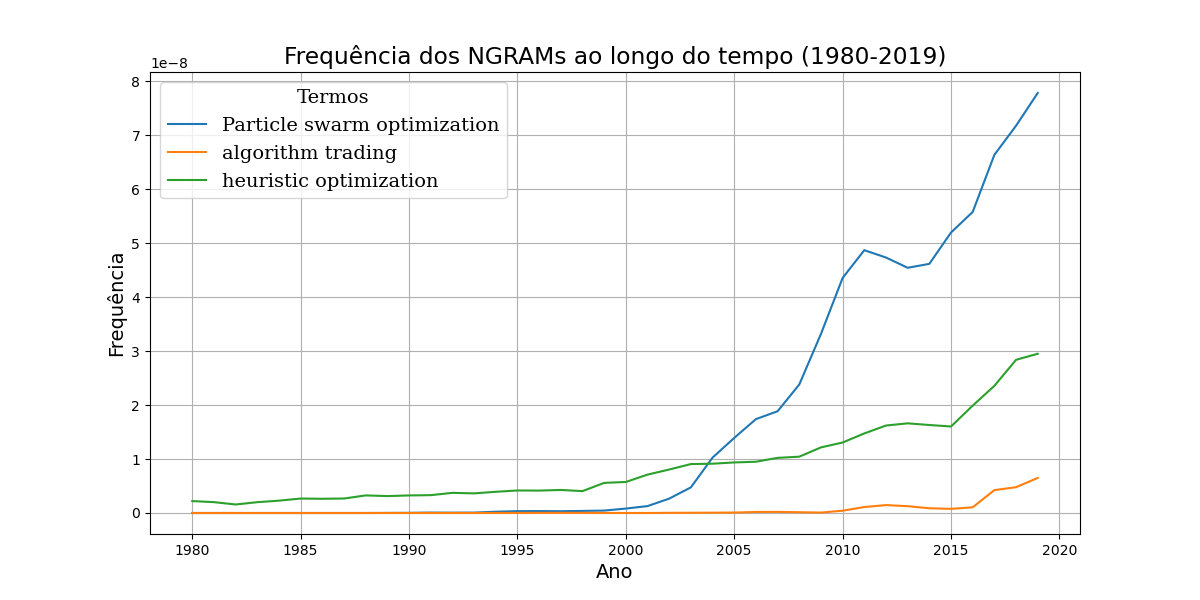
\includegraphics[width=16cm]{figuras/ngram.png}
    \legend{\citefonte{googleNgramViewer}.}
  \end{varwidth}
\end{figure}

\section{Técnicas para definição de \textit{Stop-loss} e \textit{Take-profit}}

A gestão  baseada em objetivos de perdas
e ganhos, é utilizada no mercado financeiro para um melhor gerenciamento de riscos. Nesse sentido é possível que uma operação
de compra ou venda seja encerrada ao fechar posição ao atingir um ponto de TP
ou um ponto de SL. Segundo \textcite{nametala2017construccao} a utilização de pontos de \textit{stop}
individualizados e otimizados para cada série de cada ativo é importante pois as variações
dos preços são muito específicas à cada ação. Isso é particularmente nítido quando se
observa a distribuição dos retornos de cada ativo, dessa forma ao realizar um estudo sobre
otimização de pontos de saída, chegou na proporção de 3:1, onde para TP se tem o
valor de 45\% de valorização do ativo e para SL contabilizou-se 15\% na desvalorização.

Essa proporção de 3:1 também é respaldada por outros estudos na literatura.
Em estudos como \textcite{ciniro2} e \textcite{Noertjahyana_2020}, os autores corroboram
a eficácia dessa relação, aplicando-a no contextos de mercado. Esses estudos reforçam a
ideia de que uma gestão de riscos bem estruturada, utilizando a relação de 3:1 para definir
pontos de SL e TP, pode ser uma abordagem eficaz para maximizar lucros e minimizar
perdas em operações financeiras.

\section{Trabalhos relacionados}

Alguns dos métodos utilizados envolvem a utilização de técnicas de \textit{machine
learning} para a definição de pontos de saída de operações, e estes métodos estão sendo
explorados no mercado financeiro. Segundo \textcite{Mazen2023}, os algoritmos
de aprendizado supervisionado, como o \textit{K-Nearest Neighbour} (KNN), Suporte Vetorial
(SVM), Floresta Aleatória, Redes Neurais e Árvores de Decisão, podem prever tendências
do mercado de ouro com alta precisão. Esses algoritmos foram aplicados para prever
pontos de SL e TP, obtendo-se uma acurácia de até 99\% com redes neurais. Esse modelo
adaptativo permite ajustar automaticamente os pontos de saída com base na direção do
mercado, oferecendo uma estratégia de negociação mais dinâmica e eficaz.

Outra abordagem também utilizada, é demonstrada em \textcite{Vezeris2018} que, determina 
que com indicadores técnicos como o \textit{Average True Range}
(ATR), é possível estabelecer sinais de SL e TP baseados em tendências de mercado,
proporcionando uma abordagem adaptativa que ajusta a quantidade da menor unidade de
variação do preço de uma moeda e suas posições conforme a evolução do mercado.

Além dos métodos mencionados, \textcite{8616576} propõem uma abordagem
baseada em algoritmos genéticos para a otimização de um portfólio de estratégias de
negociação em grupo (GTSP) e seus pontos de SL e TP. Esta abordagem, denominada
GTSP-SLTP, utiliza um algoritmo genético de agrupamento (GGA) para codificar e
otimizar os pontos de SL e TP em cromossomos. Cada cromossomo representa uma
combinação de estratégias de negociação, agrupamentos e pesos de capital, onde os
pontos de SL e TP são ajustados para maximizar os lucros e minimizar os riscos. Os
resultados experimentais mostram que esta técnica pode efetivamente encontrar um
portfólio otimizado e seus pontos de saída, oferecendo uma ferramenta robusta para a
gestão de risco e retorno em mercados financeiros voláteis.

Em \textcite{sivri2023}, é discutido sobre um sistema inteligente para a determinação dinâmica dos limites 
de SL e TP utilizando dados históricos de preços de ações
da IBM e análise de desvio padrão. O objetivo principal é minimizar perdas e maximizar
lucros para traders e investidores. O estudo emprega técnicas de inteligência artificial,
como algoritmos de aprendizado de máquina, para analisar os dados históricos do mercado
de ações e determinar separadamente os níveis de TP/SL para posições de compra e venda.
A eficácia da abordagem é avaliada comparando os retornos diários com os retornos dos
níveis TP/SL utilizando a métrica \textit{Sharpe Ratio}. Os resultados sugerem que a abordagem
proposta pode melhorar a precisão das estratégias de negociação automatizada, indicando
que os níveis de TP/SL determinados dinamicamente podem ser mais eficazes do que os
retornos de fechamento do dia.

A utilização de modelos LSTM (\textit{Long Short-Term Memory}) para a definição de
pontos de TP e SL tem se mostrado uma abordagem promissora no contexto de negociações
financeiras. \textcite{wu} aplica a arquitetura LSTM para prever a probabilidade de
lucro das estratégias de futuros e, em seguida, converter esses pontos de TP e SL para
operações de opções. O objetivo é melhorar a precisão e a lucratividade das estratégias
de negociação, abordando as limitações das estratégias tradicionais de futuros, como a
dificuldade em determinar o tamanho ideal das posições devido à necessidade de margem
e à volatilidade do mercado. O estudo utiliza uma rede neural LSTM para prever a
probabilidade de lucro das estratégias de futuros e, em seguida, converte os pontos diários
de TP e SL para operações de opções com base no valor delta das opções. A nova
estratégia de opções resultante é aplicada ao critério de Kelly para calcular a fração
ideal de negociação, permitindo um controle mais preciso do tamanho das posições. Os
resultados demonstram que a negociação de opções pode alcançar uma fração mais próxima
da ideal, conforme calculado pelo critério de Kelly, em comparação com a negociação de
futuros, aumentando assim a lucratividade total da estratégia.

\subsection{Diferencial da abordagem apresentada}

Em comparação com os trabalhos relacionados destacados na tabela (\ref{tab:trabalhos_relacionados}), o
diferencial deste reside na aplicação do algoritmo PSO
para a definição de pontos fixos de SL e TP no mercado financeiro. Enquanto \textcite{Mazen2023} e \textcite{wu} focam 
em técnicas de aprendizado de máquina e redes neurais
para previsão de tendências e ajustes de posições, e \textcite{8616576} utilizam algoritmos
genéticos para otimização de portfólios, a abordagem desse trabalho visa integrar a otimização por
enxame de partículas para definir os pontos de saída com base no cruzamento de médias
móveis no histórico de negociação do WINFUT. Desta forma
este trabalho oferecerá uma alternativa frente às metodologias já exploradas.

\begin{table}[htbp]
  \small
  \centering
  \begin{tabular}{|p{2.5cm}|p{3.5cm}|p{3.5cm}|p{4cm}|}
  \hline
  \textbf{Referência} & \textbf{Técnica Utilizada} & \textbf{Objetivo} & \textbf{Resultados} \\ \hline
  Mazen (2023) & Algoritmos de aprendizado supervisionado (KNN, SVM, Floresta Aleatória, Redes Neurais, Árvores de Decisão) & Plano de negociação adaptativo no mercado de ouro & Obteve-se um modelo adaptativo que permite ajustar automaticamente os pontos de saída com base na direção do mercado \\ \hline
  Vezeris, Kyrgos e Schinas (2018) & Indicadores técnicos (ATR) & Estabelecimento de sinais de SL e TP baseados em tendências de mercado & Determina que com o ATR, é possível estabelecer sinais de stop-loss e take-profit baseados em tendências de mercado \\ \hline
  Chen et al. (2018) & Algoritmo de agrupamento genético (GGA) & Otimizar um portfólio de estratégias de negociação em grupo (GTSP) utilizando pontos de \textit{stop-loss} e \textit{take-profit} & Demonstração que a abordagem proposta supera a anterior que não considerava os pontos de \textit{take-profit} e \textit{stop-loss} \\ \hline
  Sivri et al. (2023) & \textit{Random Forest, Extreme Gradient Boosting} e \textit{Light Gradient Boosting} & Determinação dinâmica dos limites de \textit{stop-loss} e \textit{take-profit} & Melhoria da métrica SP em relação ao método que calcula a difereça entre o preço de abertura e fechamento  \\ \hline
  Wu et al. (2020) & Modelos LSTM & Definição de pontos de \textit{take-profit} e \textit{stop-loss} em negociações de futuros e conversão para para operações de opções & Através do critério de Kelly a estrátegia abordada se mostrou viável devido ao aumento da lucratividade total \\ \hline
  Este trabalho & \textit{Particle Swarm Optmization} (PSO) e simulação de compras de ação utilizando cruzamento de médias móveis & Otimizar os pontos de saída nas negociações do minicontrato futuro do índice Bovespa & Obteve-se pontos de saída que perfomaram melhor que os definidos pela estratégia convencional \\ \hline
  \end{tabular}
  \caption{Comparação das técnicas e resultados de trabalhos relacionados.}
  \label{tab:trabalhos_relacionados}
  \end{table}

\chapter{METODOLOGIA}

Na primeira seção é apresentado o método de extração do histórico de negociações do ativo, o qual 
retorna informações sobre o preço do ativo a cada segundo, seguido dos procedimentos para tratar os dados obtidos, 
incluindo a interpolação de segundos faltantes. Em seguida, é descrita a fase de entrada do algoritmo PSO, 
detalhando a abordagem baseada em médias móveis utilizada para simular os pontos de compra. Também é explicado 
como o PSO foi aplicado para determinar os pontos de saída no histórico de negociações, com a descrição da implementação 
e dos parâmetros configurados. Por fim, aborda-se a metodologia para análise e comparação dos resultados obtidos. 
Todas as etapas de tratamento, padronização dos dados, geração de pontos
de compra e aplicação do PSO foram realizadas utilizando a linguagem de programação
Python no ambiente do Google Colab.

\section{Extração e tratamento de dados}

Para a realização deste trabalho, o histórico de negociação foi extraído da
plataforma \textit{home broker} \textit{Metatrader5}. Utilizou-se um \textit{script} desenvolvido na linguagem
de programação MetaQuotes Language (MQL), que gerou um arquivo no formato \textit{.csv}
contendo o valor do índice Bovespa a cada segundo, do dia 15-03-2024, dia o qual foi utilizado
para a aplicação do PSO e definição dos pontos de saída, e dos dias 18-03-2024 à 21-03-2024 para comparar 
a diferença no possível retorno utilizando a estratégia com o PSO e a estratégia que utiliza a relação 3:1.

Durante o tratamento dos dados, foi realizada uma padronização do \textit{dataset}
para garantir a consistência. Foi extraído um total de 151472 dados. O horário de início foi definido como 09:06:00 e o
de término como 17:31:00. Além disso, foi identificada a presença de 1716 duplicatas no \textit{dataset},
ou seja, registros repetidos, os quais foram removidos para evitar distorções nos resultados, fazendo que o número
de registros fosse reduzido para 149756.

Outra etapa do tratamento de dados foi a verificação de lacunas temporais, ou seja, segundos faltantes na extração do histórico,
pois durante a extração em tempo real do histórico pode ocorrer inconsistências que gerem essas lacunas.
Contabilizando todos os segundos de 09:06:00 à 17:31:00 em 5 dias de extração, seria obtido 151505 dados,
dessa forma, nota-se que houveram aproximadamente 1.15\% de dados faltantes. Para resolver essa questão,
foi aplicado a interpolação dos dados utilizando o método linear, preenchendo assim as
lacunas e garantindo a continuidade do \textit{dataset}. 

A interpolação linear é caracterizada por
atribuir o valor ao dado faltante realizando a média entre o dado seguinte e o dado anterior,
onde na aplicação em questão, a interpolação é feita atribuindo o valor ao segundo faltante
$x$ através da realização da média entre os valores nos dois segundos mais próximos, o valor
segundo anterior $x-1$ e o valor do segundo seguinte $x+1$.

\section{Fase de entrada do PSO}

Com os dados já tratados foi possível realizar as simulações de compra utilizando
as médias móveis. A partir das simulações de compra dos dados extraídos no dia 15-03-2024, foi aplicado 
o PSO de forma a definir o TP e SL que possibilitariam um maior retorno na data em questão. 
A estratégia utilizada para a simulação de compra foi uma variação da
técnica abordada em \textcite{PAPAILIAS2015458}, que descreve uma estratégia através da
emissão de um sinal de compra quando uma média móvel mais rápida cruza acima de
uma média móvel mais lenta e a emissão de sinais de venda quando ocorrer
o oposto, a estratégia utilizada neste trabalho considera apenas a emissão do sinal de
compra, desconsiderando o sinal de venda.

Para a aplicação do PSO, primeiramente é definido uma função, que percorre os dados tratados
anteriormente, contendo os preços, e gera duas médias móveis de diferentes períodos,
uma de 9 e outra de 21. Logo em seguida os dados são percorridos novamente, porém
comparando as duas médias móveis geradas para cada segundo. Quando a média móvel
de curto prazo (mm9) cruza acima da média móvel de longo prazo (mm21), é registrado
o sinal de compra para o segundo correspondente, indicando o cruzamento. Por fim, os
dados são exportados para um arquivo \textit{.csv}, contendo os preços e os sinais de compra,
facilitando a análise subsequente.

\section{Aplicação do PSO}

Para realizar a aplicação do PSO, primeiramente foi preciso implementar uma
função capaz de calcular o retorno das operações de compra utilizando o TP e SL como
parâmetros na função. A função deve ser capaz de simular uma compra ao encontrar o
sinal de compra no ponto $c$ e simular uma venda ao atingir o TP ou o SL no ponto $v$, e
dessa forma calcular qual foi o retorno obtido nessa compra através da subtração entre o
valor do ativo no ponto $v$ e o valor do ativo no ponto $c$. Ao percorrer todo o histórico de
negociações a função retornará o somatório de todos os retornos de cada ponto de compra.

A abordagem de SL e TP deste trabalho utiliza a variação do
preço de compra em pontos, onde a variação de cada ponto indica uma variação de 5 reais
no preço do ativo.

O próximo passo será implementar a função objetivo que irá utilizar a função
de cálculo de retorno das operações. A função objetivo calcula o retorno para os pontos
de SL e TP definidos por cada possível particula do PSO.

A função objetivo, que busca maximizar o lucro das operações de compra e venda com base nos parâmetros \textit{Take-Profit} (TP) e \textit{Stop-Loss} (SL), pode ser expressa como:

\begin{equation}
f(x) = \sum_{i=1}^{n} \left( \text{retorno}_{i} \right),
\end{equation}

onde \( x = (TP, SL) \) representa os valores de TP e SL otimizados para cada 
partícula do PSO, e o retorno de cada operação \( i \) da abordagem utilizada, é dado por:

\begin{equation}
\text{retorno}_{i} =
\begin{cases} 
p_{v} - p_{c}, & \text{se } p_{v} \geq p_{c} + (5 \cdot TP) \text{ ou } p_{v} \leq p_{c} + (5 \cdot SL), \\
0, & \text{caso contrário}.
\end{cases}
\end{equation}

Onde:
\begin{itemize}
    \item \( p_{c} \) é o preço de compra no ponto de sinal \( c \),
    \item \( p_{v} \) é o preço de venda no ponto \( v \),
    \item \( n \) é o número total de operações realizadas.
\end{itemize}

Com essas funções já implementadas, foi possível realizar a aplicação do PSO
para o problema em questão. Na implementação realizada, foi utilizado o \textit{GlobalBestPSO}
da biblioteca \textit{pyswarms} \cite{miranda2018pyswarms}. Esta função define os parâmetros ótimos da função objetivo de
maneira a minimizar o valor retornado. Como o objetivo em questão foi definir os pontos de
saída para aumentar o retorno, então foi necessário fazer uma alteração na função objetivo
de forma que o retorno seja multiplicado por -1. Desta forma, a função PSO utilizada irá
definir os pontos de saída que maximizem o retorno.

Para aplicar a função \textit{GlobalBestPSO} é necessário definir os parâmetros coeficiente 
de aceleração cognitiva $c1$, coeficiente de aceleração social $c2$, fator de inércia
$w$, limites inferiores, limites superiores, número de partículas, número de dimensões e
números de iterações. Estes parâmetros afetam a maneira com que os valores ótimos são
encontrados na função objetivo. Enquanto os limites influenciam nos valores máximos e
mínimos que as partículas podem retornar, os valores $c1$, $c2$ e $w$, influenciam na dinâmica
de movimentação das partículas, determinando o equilíbrio entre a exploração do espaço
de busca e a exploração local em torno das melhores soluções encontradas. A dimensão
altera a quantidade de valores que cada particula retorna. Os seguinte parâmetros foram
utilizados na aplicação do PSO:

\begin{itemize}
  \item c1: 0.5
  \item c2: 0.3
  \item w: 0.9
  \item Número de dimensões: 2
  \item Limites inferiores: [1, 1]
  \item Limites superiores: [25, 25]
  \item Número de particulas: 30
  \item Número de iterações: 100
\end{itemize}

O número de partículas (30) e o número de iterações (100) foi escolhido levando em consideração o tempo de execução e a 
eficiência da busca. Já os parâmetros 
c1, c2 e w foram definidos com base em outras implementações do PSO. Os limites 
estabelecidos foram definidos considerando uma variação mínima de 5 reais e uma variação máxima próxima de 125 reais. 
Esses limites foram definidos de forma a simular um ambiente que busca obter ao menos um lucro mínimo, sem 
arriscar tanto a ponto de perder uma quantia significativa em uma única negociação.

\section{Análise e comparação entre abordagens}

Após a aplicação do PSO, os pontos de saída
foram definidos, a partir desses, será feito uma análise do retorno que
teria sido obtido nos 4 dias de operação seguintes ao dia em que o PSO foi aplicado. Nessa análise, será considerado as
abordagens apresentadas a seguir:

A abordagem do trabalho consiste em definir os pontos de saída com base em variações no preço de compra por meio da 
aplicação do algoritmo PSO, em que cada ponto corresponde a uma variação de 5 reais, 
que é a variação mínima do preço de um ativo na B3. Em contrapartida, a abordagem comumente utilizada considera a 
proporção de 3:1, respaldada por estudos presentes na literatura. Nessa abordagem, os valores de TP e SL foram definidos 
de forma próxima aos valores obtidos pelo PSO, mas ajustados para respeitar a relação de 3:1.

Após a apresentação dos retornos, será mostrado em gráfico, as operações que teriam sido
realizadas por cada abordagem nos 4 dias de operações seguintes ao dia em que foi aplicado o PSO,
utilizando os mesmos pontos de saída. 

\chapter{RESULTADOS}

Este capítulo está dividido em duas seções. Na primeira seção é apresentado sobre os 
pontos de saída obtidos com a aplicação do PSO no histórico de negociações
do dia 15-03-2024. Na segunda seção está o comparativo entre as operações que seriam
efetuadas em cada abordagem no período dos dias 18, 19, 20 e 21 de março de 2024.

\section{Pontos de saída obtidos}

Com a aplicação da técnica de compra baseada em cruzamento de médias
móveis, foram obtidos 55 sinais de compra. Com a aplicação do PSO foi possível obter
pontos de saída das operações de compra que maximizassem o lucro a ser obtido. A seguir
é apresentado os pontos de saída obtidos com aplicação do PSO e os que foram utilizados
na abordagem que considera a relação 3:1.

\begin{itemize}
  \item Abordagem PSO:
      \begin{itemize}
          \item Unidade: Variação em pontos em relação ao preço de compra
          \item \textit{Take Profit} (TP): 2.0882
          \item \textit{Stop Loss} (SL): 13.0824
      \end{itemize}
  \item Abordagem 3:1:
      \begin{itemize}
          \item Unidade: Variação em pontos em relação ao preço de compra
          \item \textit{Take Profit} (TP): 6
          \item \textit{Stop Loss} (SL): 2
      \end{itemize}
\end{itemize}

\section{Comparação entre abordagens}

Após realizar a simulação de compra utilizando a técnica de cruzamento
de médias móveis, juntamente com os pontos de saída definidos em cada abordagem,
obteve-se a variação do retorno. O
retorno por dia é demonstrado na tabela (\ref{tab:retornoDia}) e o retorno acumulativo por dia é demonstrado na tabela (\ref{tab:retornoAcumulativoDia}).


\begin{table}[!htb]
  \caption{Retorno por dia} \label{tab:retornoDia}
  \begin{tabularx}{\textwidth}{X|r|r} 
  \hline
  Data     & Abordagem PSO (R\$) & Abordagem 3:1 (R\$) \\ 
  \hline
  18-03-2024 & 4785,83     & -781,66    \\
  19-03-2024 & 2215,00     & -725,00      \\
  20-03-2024 & 3240,00     & 345,00       \\ 
  21-03-2024 & -457,50     & -2820,00 \\
  \hline
  \end{tabularx}
  \legend{Elaborado pelo Autor, 2024.}
\end{table}

\begin{table}[!htb]
  \caption{Retorno acumulativo por dia} \label{tab:retornoAcumulativoDia}
  \begin{tabularx}{\textwidth}{X|r|r} 
  \hline
  Data     & Abordagem PSO (R\$) & Abordagem 3:1 (R\$) \\ 
  \hline
  18-03-2024 & 4785,83     & -781,66    \\
  19-03-2024 & 7000,83     & -1506,66      \\
  20-03-2024 & 10240,83    & -1161,66      \\ 
  21-03-2024 & 9783,33     & -3981,66 \\
  \hline
  \end{tabularx}
  \legend{Elaborado pelo Autor, 2024.}
\end{table}

Como visto nas tabelas, a abordagem que faz uso do PSO resultou
em um retorno total positivo, o que indica uma boa performance nos resultados obtidos. Em contraste, a abordagem
que adota uma relação de 3:1 entre TP e SL, revelou um
desempenho significativamente inferior, resultando em 3 dias com retornos negativos e apenas um dia
com retorno positivo, finalizando com um retorno negativo de R\$3981,66 reais. Esse
resultado destaca uma discrepância importante em relação a abordagem que utiliza os pontos definidos pelo PSO e sugere
que a configuração da relação de 3:1 impacta negativamente os resultados quando a estratégia
adotada para compra é a de médias móveis. 

Nos gráficos a seguir, é apresentado o retorno
acumulativo por operação, eles ilustram que variação dos retornos apresentam um
padrão semelhante para as abordagens que fazem uso dos pontos de saída definidos
pelo PSO, sugerindo que ambas têm um comportamento análogo em termos de desempenho.

\begin{figure}[!htb] \centering
    \caption{Variação do retorno - Abordagem PSO} \label{figura:vreta2}
    \begin{varwidth}{\linewidth}
        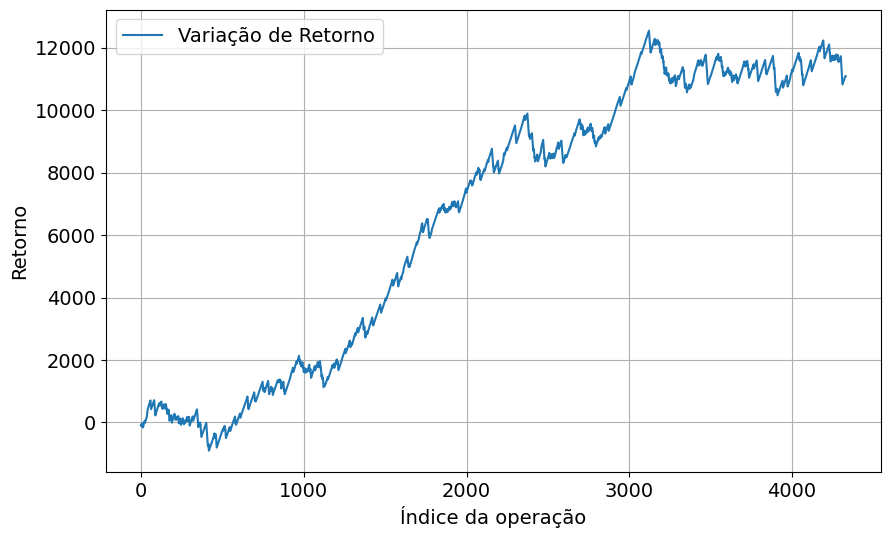
\includegraphics[width=14cm]{figuras/abordagem2.png}
        \legend{Elaborado pelo Autor, 2024.}
    \end{varwidth}
\end{figure}

\begin{figure}[H] \centering
    \caption{Variação do retorno - Abordagem 3:1} \label{figura:vreta3}
    \begin{varwidth}{\linewidth}
        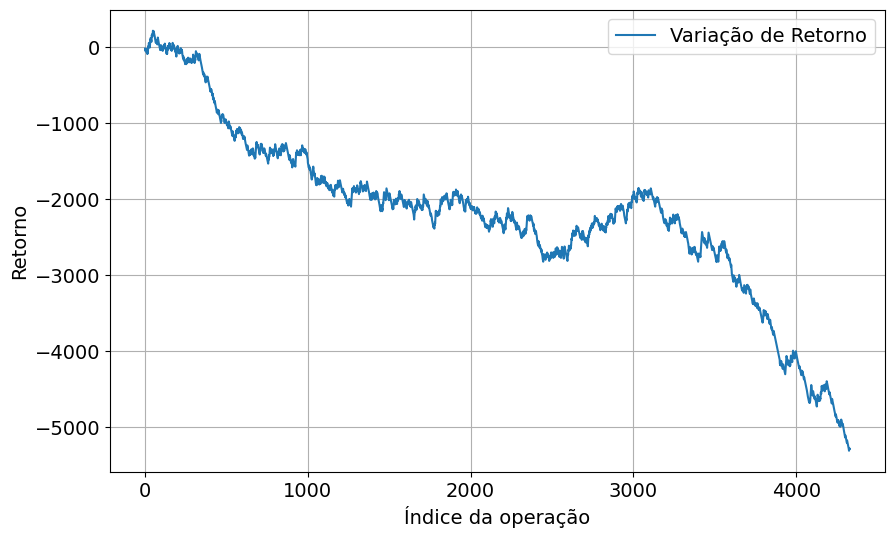
\includegraphics[width=14cm]{figuras/abordagem3.png}
        \legend{Elaborado pelo Autor, 2024.}
    \end{varwidth}
\end{figure}

Ao calcular a diferença total entre as abordagens, observa-se que o retorno acumulativo final da abordagem PSO foi 
de R\$9783,33, enquanto a abordagem 3:1 apresentou um saldo final de -R\$3981,66, resultando em uma diferença total 
de R\$13.764,99 a favor da abordagem PSO. Esse resultado demonstra de forma clara e objetiva que a aplicação do PSO 
para definição dos pontos de saída proporciona um desempenho substancialmente superior. A abordagem PSO não apenas 
evitou os prejuízos observados na abordagem 3:1, mas também maximizou consistentemente os lucros, consolidando-se 
como a melhor escolha no contexto analisado.

\chapter{CONCLUSÃO}

Durante este trabalho foi feita a aplicação do PSO para definição dos pontos
de TP e SL em negociações envolvendo o minicontrato futuro do índice Bovespa. Para
realizar tal trabalho, foi extraído um \textit{dataset} contendo o histórico de negociações, nos dias 
15, 18, 19, 20 e 21 de março de 2024. Após a extração, etapas como tratamento
e padronização de dados foram realizadas, de forma a contríbuir para a consistência e a
continuidade dos dados. 

Com os dados já tratados, foi feita uma simulação de compra
no \textit{dataset}, considerando a estratégia de cruzamento de médias móveis. Com isso, foi
estipulada uma função objetivo que calcula o lucro a ser obtido na simulação de compra
baseado nos pontos de saída. Tendo essa função objetivo implementada, foi aplicado o
algoritmo de otimização meta-heurístico PSO à simulação de compra no dia 15 utilizando
a função objetivo, de forma a definir os pontos ótimos de TP e SL para maximizar o
lucro. A partir dessa aplicação foram feitas análises e comparações entre duas
abordagens de pontos de saída.

Através das análises ficou demonstrado que o método proposto neste trabalho mostrou ser eficaz na
identificação de pontos estratégicos de TP e SL, pois a abordagem que faz uso do PSO
mostrou ser robusta e consistente, de forma a demonstrar obtenção de lucro em 3
dias de negociação. Em contrapardita a abordagem que considera a relação 3:1 observada em trabalhos acadêmicos e
em plataformas de negociação, apresentou resultados inferiores nos dias analisados.
Esses resultados indicam que a escolha adequada dos parâmetros de TP e SL é crucial
para a maximização dos lucros em operações de mercado e que o método aplicado para a
definição desses pontos é valido e eficaz.

Com base nos resultados obtidos e nas análises realizadas, um próximo passo
pode ser considerado para aprimorar a avaliação da estratégia de negociação e validar as
conclusões. Este passo se baseia em utilizar uma plataforma de negociação para realizar
operações fictícias com o WINFUT, fazendo uso da estratégia
de cruzamento de médias móveis para compra do ativo, e o uso dos pontos de saída
definidos com a aplicação do PSO.


\chapter*{REFERÊNCIAS}

\printbibliography

\end{document}
